%This template has been used to publish the thesis of Buijs~\cite{MScBuijs2010} and is originally used for the thesis of Nugteren~\cite{MScNugteren2010}. 

%One of the best resources for \LaTeX basics, and advanced constructs, is the \LaTeX wikibook\footnote{To be found at~\url{http://en.wikibooks.org/wiki/LaTeX/}}. Of course colleagues and a good internet search using your favorite search engine can do wonders if you're stuck. 

In this chapter, we describe the related state-of-the-art and widely used deep learning architecture for image processing. The datasets that will be used for experiment will also explained in this section.  


%Traditional machine learning technique such as SVM and  suffers from high-dimensional data such as voice and image. 


\section{Deep Learning}
Deep learning is a special form of neural networks that uses complex model to solve a problem. Deep learning technique that heavily used for dealing with image classification problem is convolutional neural network (CNN). In CNN, usually the model goes into three kinds of layers (other than the input and output layers).

The first layer type is convolutional layer. In this layer an element wise multiplication operation is implemented using a moving kernel/filter. A convolutional layer produces some feature maps for the next process. The output of the convolutional layer is usually connected to an activation function such as ReLU, tanh or sigmoid. The second type of layer is subsampling/pooling layer. This layer's function is to reduce the number of tuned parameters. The common operators for subsampling layer are: max-pooling and average pooling. The last type is fully-connected layers. In this layer, the networks try to determine the probability of the input falls into each class by learning the high level abstraction from convolutional and maxpooling layer output. There is also an optional layer that serves as regularization layer such as dropout layer. There are a lot of deep learning architecture that was proposed. Below, we highlight some of the most interesting architecture to be tested in the experiment. 
\subsection{LeNet-5}
LeNet-5 was proposed by Yann LeCun, et al. \cite{lecun1998gradient} consists of seven non-input layers 
The first layer is a 5x5 convolutional layer with six feature maps. The second layer is a 2x2 non-overlapping subsampling layer. The third layer is a 5x5 convolutional layer with sixteen feeature maps. The fourth layer consists of 2x2 non-overlapping subsampling layer. The fifth layer is a 5x5 convolutional layer with 120 feeature maps. The sixth layer is an 84-units fully-connected layer. The output layer is composed of Euclidean RBF units, one for each class, with 84 inputs each. The architecture of LeNet-5 can be seen in figure \ref{fig:lenet5}. LeNet-5 is one of the first initial architectures of CNN that was tested to classify hand-written number using MNIST dataset.


\begin{figure}[h]
	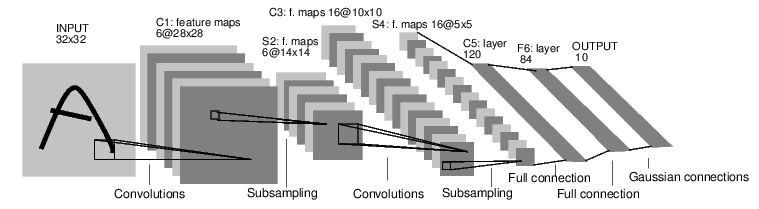
\includegraphics[scale=0.5]{figures/lenet5}
	\centering
	\caption{LeNet-5 Architecture \cite{lecun1998gradient}}
	\label{fig:lenet5}
\end{figure}


\subsection{Alex-Net}
Alex Net was proposed by Alex Krizhevsky, et al. \cite{krizhevsky2012imagenet} based on their winning on ILSVRC (ImageNet Large-Scale Visual Recognition Challenge) 2012. The architecture consists of eight layers: five convolutional and three fully-connected layers. The first convolutional layer is using a 11x11 filter size with a stride of 4. The other convolutional layer use 3x3 filter size. The subsampling layer that was used is max-pooling. An architecture of Alex-Net can be seen in figure \ref{fig:alexnet}. It was tested on ILSVRC 2012 dataset and achieves top 5 test error rate of 15.4\%.
\begin{figure}[h]
	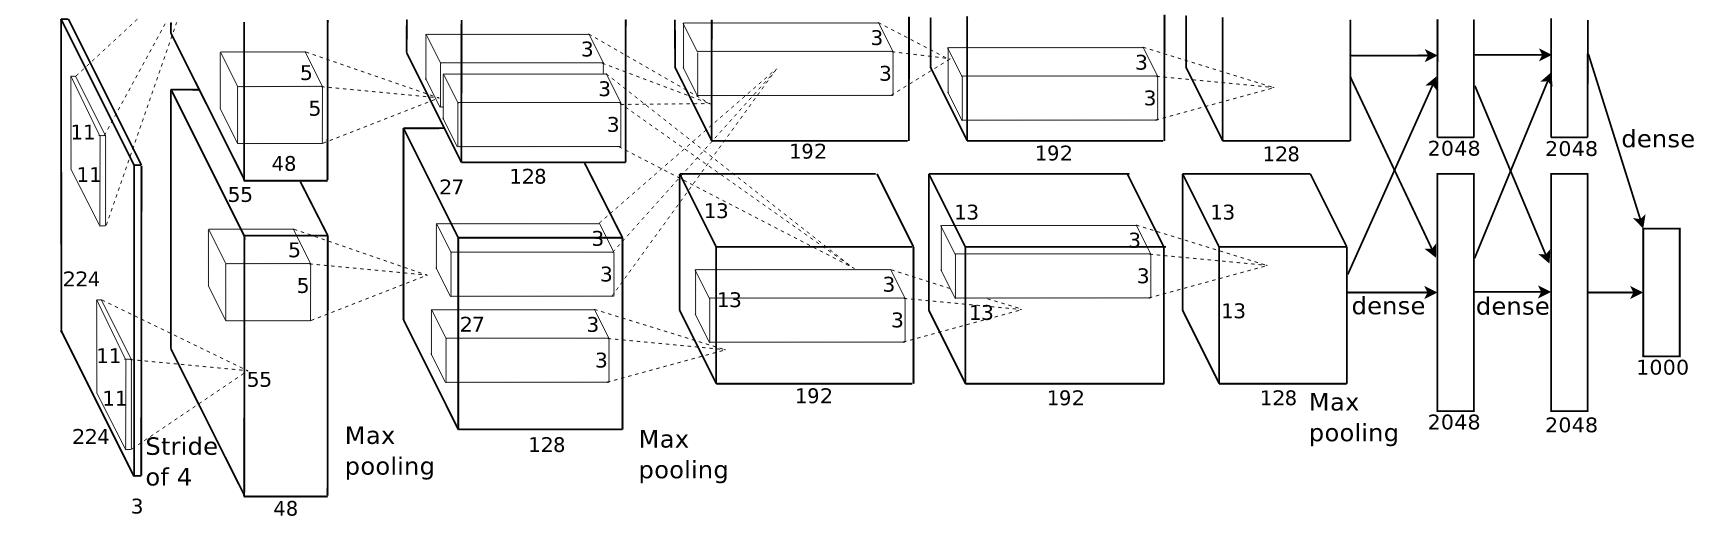
\includegraphics[scale=0.25]{figures/alexnet}
	\centering
	\caption{Alex Net Architecture \cite{krizhevsky2012imagenet}}
	\label{fig:alexnet}
\end{figure}
%\subsection{ZF-Net}
%ZF-Net was proposed by Zeiler and Fergus \cite{zeiler2014visualizing}. It was the winner of ILSVRC 2013. ZF-Net is a modification from Alex-Net. One of the differences between ZF-Net and Alex-Net is the filter size in the first layer, instead of using 11x11 with stride 4 like Alex-Net did, ZF-Net using 7x7 filter size with stride 2. The full architecture of ZF-Net can bee seen in figure \ref{fig:zf}. It was tested on the ILSVRC 2012 dataset and achieved 11.2\% error rate.

%\begin{figure}[h]
%	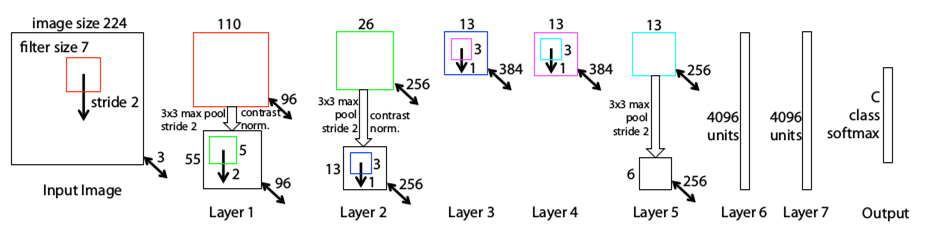
\includegraphics[scale=0.5]{figures/zfnet}
%	\centering
%	\caption{ZF Net Architecture \cite{zeiler2014visualizing}}
%	\label{fig:zf}
%\end{figure}


\subsection{VGG Net}
VGG Net was proposed by Karen Simonyan and Andrew Zisserman \cite{simonyan2014very} based on their winning on ILSVRC 2014. The architecture has 6 variations as shown in figure \ref{fig:vgg}. The key idea of this architecture is using a 3x3 filter size with a stride of 1 for every convolutional layer. In subsampling layer, VGG-Net uses 2x2 max pooling layer with stride size of 2. It was tested on ILSVRC-2012 dataset and can achieve a top-5 test error of 6.8\%.

\begin{figure}[h]
	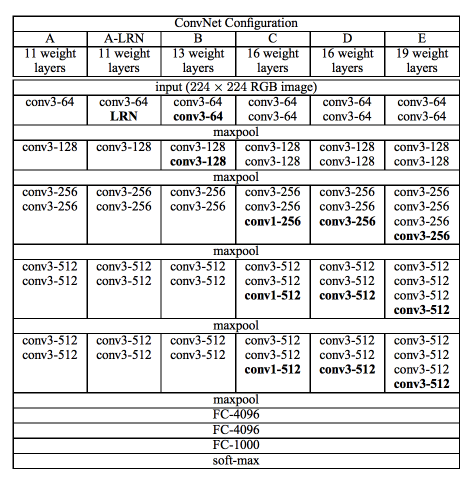
\includegraphics[scale=0.5]{figures/vggnet}
	\centering
	\caption{VGG Net Configuration \cite{simonyan2014very}}
	\label{fig:vgg}
\end{figure}


\subsection{ResNet}
In 2015, Microsoft proposed a very deep architecture called ResNet \cite{he2016deep}. It can go up to 1202 layers, but the best results for CIFAR-10 dataset is 6.43\% error rate by using 110 layers. The idea behind ResNet is stacking convolutional layer with 3x3 filter size until it reaches a very deep network.  

%\subsection{Simple Net}

\section{Dataset}
Benchmarking the proposed deep learning architecture can be done by collecting some datasets to evaluate the architecture that was presented before. Here we presents some interesting image datasets.
\subsection{MNIST}
The MNIST Datasets (http://yann.lecun.com/exdb/mnist/) is a dataset of handwritten digits with 784 features (28x28 grayscale images). There are 10 classes, 60,000 training examples and 10,000 testing examples. An example of MNIST dataset can be seen in figure \ref{fig:mnist}.

We choose this dataset because it is heavily used as validation datasets for image recognition learning algorithm. Also it doesn't need preprocessing and formatting steps since the data is quite clean, thus we can focus on the learning implementation.

\begin{figure}[h]
	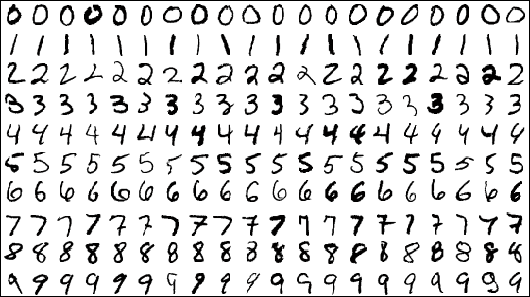
\includegraphics[scale=0.3]{figures/mnist}
	\centering
	\caption{An example of MNIST dataset}
	\label{fig:mnist}
\end{figure}

\subsection{Fashion-MNIST}
Fashion-MNIST \cite{xiao2017/online} is a dataset of Zalando's article images consisting of a training set of 60,000 examples and a test set of 10,000 examples. Each example is a 28x28 grayscale image, associated with a label from 10 classes. Zalando intends Fashion-MNIST to serve as a direct drop-in replacement for the original MNIST dataset for benchmarking machine learning algorithms. It shares the same image size and structure of training and testing splits.

Compared to MNIST, this datasets are quite new. Thus, unlike MNIST, these datasets are not heavily studied. We choose this datasets because of the similarities with MNIST datasets in terms of image size and representation. 
\begin{figure}[h]
	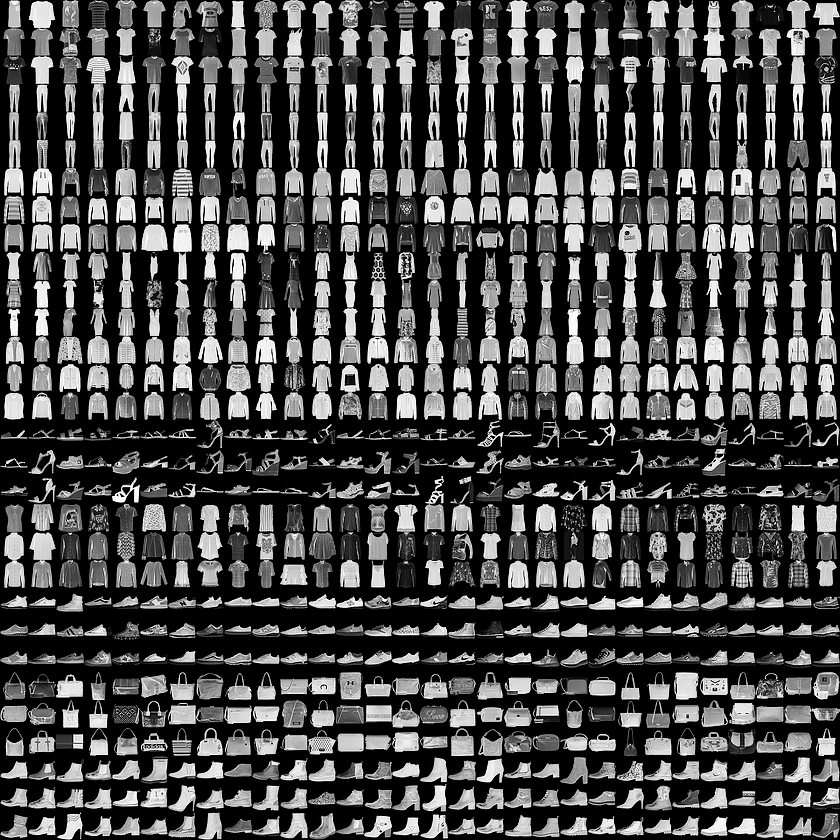
\includegraphics[scale=0.3]{figures/fashion-mnist}
	\centering
	\caption{Fashion-MNIST sprite. Each three rows in the sprite corresponds to a single class example. \cite{xiao2017/online}}
	\label{fig:fashionmnist}
\end{figure}

\subsection{CIFAR-10}
CIFAR-10 is a labeled subset of the 80 million tiny images dataset that were collected by Alex Krizhevsky, Vinod Nair, and Geoffrey Hinton \cite{krizhevsky2009learning}. It consists of 32x32 color images representing 10 classes of objects: airplane, automobile, bird, cat, deer, dog, frog, horse, ship, truck. An example of CIFAR-10 dataset can be seen in figure \ref{fig:cifar10}.

CIFAR-10 contains 6000 images per class. The original train-test split randomly divided these into 5000 train and 1000 test images per class.
The classes are completely mutually exclusive. For example, there is no overlap between automobiles and trucks. "Automobile" includes sedans, SUVs, things of that sort. "Truck" includes only big trucks. Neither includes pickup trucks.



\begin{figure}[h]
	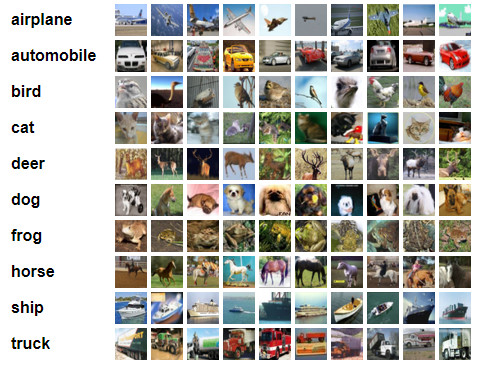
\includegraphics[scale=0.5]{figures/cifar10}
	\centering
	\caption{Example of CIFAR-10 dataset \cite{krizhevsky2009learning}}
	\label{fig:cifar10}
\end{figure}

%\subsection{CIFAR-100}
%CIFAR-100 \cite{krizhevsky2009learning} dataset is just like the CIFAR-10, except it has 100 classes containing 600 images each. There are 500 training images and 100 testing images per class. The 100 classes in the CIFAR-100 are grouped into 20 superclasses. Each image comes with a "fine" label (the class to which it belongs) and a "coarse" label (the superclass to which it belongs).

%\subsection{STL-10}
%STL-10 dataset \cite{coates2011analysis} is an image recognition dataset that were acquired from labeled examples on ImageNet. It is inspired by the CIFAR-10 dataset but with some modifications. In particular, each class has fewer labeled training examples than in CIFAR-10, but a very large set of unlabeled examples is provided to learn image models prior to supervised training. The primary challenge is to make use of the unlabeled data (which comes from a similar but different distribution from the labeled data) to build a useful prior. We also expect that the higher resolution of this dataset (96x96) will make it a challenging benchmark for developing more scalable unsupervised learning methods.

%There are 10 classes in this dataset: airplane, bird, car, cat, deer, dog, horse, monkey, ship, truck. Each images are colored 96x96 pixels.
%500 training images (10 pre-defined folds), 800 test images per class.
%100000 unlabeled images for unsupervised learning. These examples are extracted from a similar but broader distribution of images. For instance, it contains other types of animals (bears, rabbits, etc.) and vehicles (trains, buses, etc.) in addition to the ones in the labeled set.


%\begin{figure}[h]
%	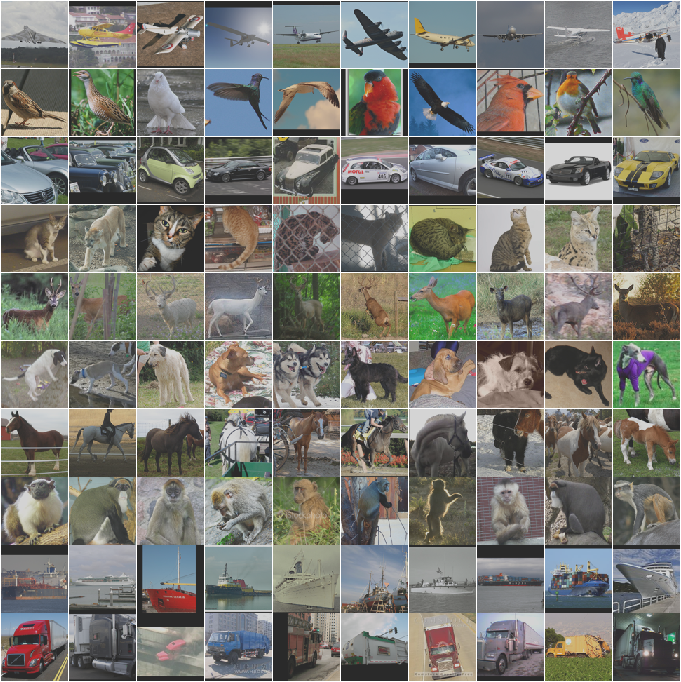
\includegraphics[scale=0.3]{figures/stl}
%	\centering
%	\caption{Examples of STL-10 datasets \cite{coates2011analysis}}
%	\label{fig:svhn}
%\end{figure}

\subsection{SVHN}
The Street View House Numbers (SVHN) Dataset \cite{netzer2011reading} is a dataset obtained from house numbers in Google Street View images. It is similar to MNIST (e.g., the images are of small cropped digits), but incorporates an order of magnitude more labeled data (over 600,000 digit images) and comes from a significantly harder, unsolved, real world problem (recognizing digits and numbers in natural scene images).

There are 10 classes, 73257 digits for training, 26032 digits for testing, and 531131 additional, somewhat less difficult samples, to use as extra training data. There are two formats of this datasets. The one that we are consider is the second format which is an MNIST-like dataset with 32-by-32 images centered around a single character (many of the images do contain some distractors at the sides).

\begin{figure}[h]
	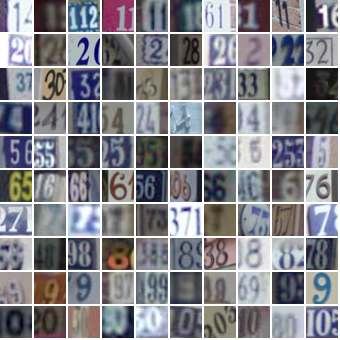
\includegraphics[scale=0.5]{figures/svhn}
	\centering
	\caption{Examples of SVHN datasets \cite{netzer2011reading}}
	\label{fig:svhn}
\end{figure}

